%! Mode:: "TeX:UTF-8"
%! TEX program = xelatex
\PassOptionsToPackage{quiet}{xeCJK}
\documentclass{cumcmthesis} %  cls 文件

% --- 仅加载 .cls 文件中【未包含】的、本文档【特有】的宏包 ---
\usepackage[numbers,sort&compress]{natbib}    % 文献管理


% --- 论文和个人信息 ---

\title{基于xxxx}
\studentid{24103219}
\studentname{贺江阳}
\college{人工智能学院}
\major{软件工程}

%%%%%%%%%%%%%%%%%%%%%%%%%%%%%%%%%%%%%%%%%%%%%%%%%%%%%%%%%%%%%
%% 正文
\begin{document}

% 显示封面
\maketitle

%摘要
% 摘要页
\begin{abstract}

开始摘要的主要内容

\keywords{几何体归类 \quad 刚性配准 \quad 多尺度特征提取 \quad Kabsch算法 \quad 迭代最近点(ICP)算法}

\end{abstract}

% 添加目录页
\cleardoublepage % 或者 \newpage,确保从新的一页开始
                 % \cleardoublepage 更好,因为它会处理好奇偶页

\pagestyle{empty}    % <--- 从这里开始,所有后续页面的样式都为空(无页眉页脚)
\tableofcontents     % 生成目录 (可能会跨越多页,所有这些页都将是 empty 样式)

\cleardoublepage     % 结束目录页,并确保下一页是奇数页,同时也让 empty 样式到此为止
\pagestyle{plain}    % <--- 恢复页面样式为 plain (通常页码在底部居中)
                     % 如果你的模板有特定的正文页面样式,例如 'headings',这里用那个

%各部分
\section{问题的提出}
\subsection{问题的重述}
在此处重述赛题问题。例如:
××××××问题就是要解决××××××××××××事情。
本文将要解决以下几个问题:

\textbf{问题一} (将论文题目的问题一摘抄过来即可)

\textbf{问题二} (将论文题目的问题二摘抄过来即可)

\textbf{问题三} (将论文题目的问题三摘抄过来即可)

\subsection{研究背景}
\subsubsection*{(1) 研究意义} % 使用无编号的subsubsection以匹配a.txt格式
% 结合题目和资料, 交代一下研究问题的重要性\研究意义.(字数不要太多,200-400左右.)
在此处填写研究意义。××××××

\subsubsection*{(2) 参考文献综述}
几何体归类与点集配准问题已有多年研究历史。Kabsch\cite{kabsch1976solution}在1976年提出了一种通过最优旋转关联两组点集的算法,成为点集刚性配准的基础方法。Besl和McKay\cite{besl1992method}在1992年提出的迭代最近点(ICP)算法进一步解决了点集间的配准问题,广泛应用于三维形状匹配。Mardia和Kent\cite{mardia1987procrustes}发展了Procrustes分析方法用于形状的统计分析。近年来,Chen等人\cite{chen2015robust}和Ma等人\cite{ma2014robust}提出了一系列基于向量场一致性和稀疏空间共识的鲁棒特征匹配方法,提高了点集匹配在噪声和异常值存在情况下的精度。Zhang等人\cite{zhang2020recent}对点云配准的几何方法和基于学习的方法进行了全面综述。这些研究为本文构建多尺度特征与刚性配准结合的几何体归类判别模型提供了重要理论基础和技术支持。




\section{问题的分析}
%    对本文提出的××××问题,我逐一做如下分析:
% (注意:问题分析主要起承上启下的作用. 不要写太冗长.)
对本文提出的××××问题,我逐一做如下分析:

\textbf{问题一的分析:}分析一下解决问题一需要注意什么, 做怎样的模型假设, 什么理由. 大致说明问题用一什么方法求解. 

\textbf{问题二的分析:}分析一下解决问题二需要注意什么, 做怎样的模型假设, 什么理由. 交代一下问题二和问题一有什么联系. 大致说明问题二用什么方法求解.

\textbf{问题三的分析:}分析一下解决问题三需要注意什么, 做怎样的模型假设, 什么理由. 交代一下模型三和前面模型有什么联系. 大致说明问题三用什么方法求解.


\section{模型假设}
根据本文提出的问题和以上的问题分析,为确保后续模型构建的科学性和结果的有效性,我们做了如下关键模型假设:

\begin{enumerate}
    \item ××××××××
    \item ××××××××
    \item ××××××××
    \item ××× % 根据需要增删
\end{enumerate}
\section{符号说明}
本文常用符号见下表,其它符号见文中说明。

\begingroup % 开始局部作用域
\setlength{\heavyrulewidth}{2.5pt} % 设置希望的粗细,仅在此组内有效

\begin{table}[H]
\centering
\caption{符号说明表}
\begin{tabularx}{\textwidth}{CCC}
\toprule % 这条线会使用上面设置的 1.2pt
\textbf{符号}    & \textbf{说明}    & \textbf{单位} \\
\midrule % 中间线的粗细 (由 \lightrulewidth 控制) 保持不变
\textbf{$P$, $Q$} & \textbf{点集} & \textbf{-} \\
$p_i$, $q_i$ & 点集中的点 & - \\
$R$ & 旋转矩阵 & - \\
$t$ & 平移向量 & - \\
$RMSD$ & 均方根偏差 & - \\
$\mathbf{c}$ & 重心 & - \\
$d_{ij}$ & 点$i$与点$j$之间的距离 & - \\
$\theta_i$ & 内角 & 弧度 \\
$\mathcal{F}$ & 特征向量 & - \\
$\lambda$ & 阈值参数 & - \\
$\delta$ & 形变参数 & - \\
$\sigma$ & 噪声强度 & - \\
\bottomrule % 这条线也会使用上面设置的 1.2pt
\end{tabularx}
\label{tab:符号说明}
\end{table}

\endgroup % 结束局部作用域,\heavyrulewidth 恢复到之前的值
\section{建模与求解}
% 简单陈述主要内容, 比如
% 这里将通过数学建模,讨论\解决本文所提出的X个问题。共分为X个小节。
% 或者
% 在这里,讨论本文所提出的X个问题解答,对每个问题分别进行数学建模与模型求解。共分为X个小节。
这里将通过数学建模,讨论并解决本文所提出的 X 个问题。共分为 X 个小节。

\subsection{问题一的建模与求解}
% 简短的概述, 问题一主要要解决什么问题, 建立了××××××模型, 用了什么方法解决. 
% 写出本小节主要内容(比如:本小节主要内容是数据的预处理、××××××模型的建立、模型的求解和分析、模型检验). 
问题一主要解决 ×××××× 问题,为此建立了 ×××××× 模型, 采用了 ×××××× 方法进行求解。
本小节主要内容包括:数据的预处理、××××××模型的建立、模型的求解和分析、模型检验或修正。

\subsubsection{数据的预处理(如果是做数据多的题, 一定要写这一块; 不需要的就不做.)}
    \textbf{1. 数据的采集}
    
    ××××××××
    
    \textbf{2. 去噪处理}
    
    ××××××××
    
    \textbf{3. 数据的整理(如不全的数据要补全, 有的是要转化数据类型, 等等)}
    
    ××××××××

\begin{figure}[H] % [H] 选项来自 float 宏包,表示将图片"确实放在这里"
    \centering      % 图片居中显示
    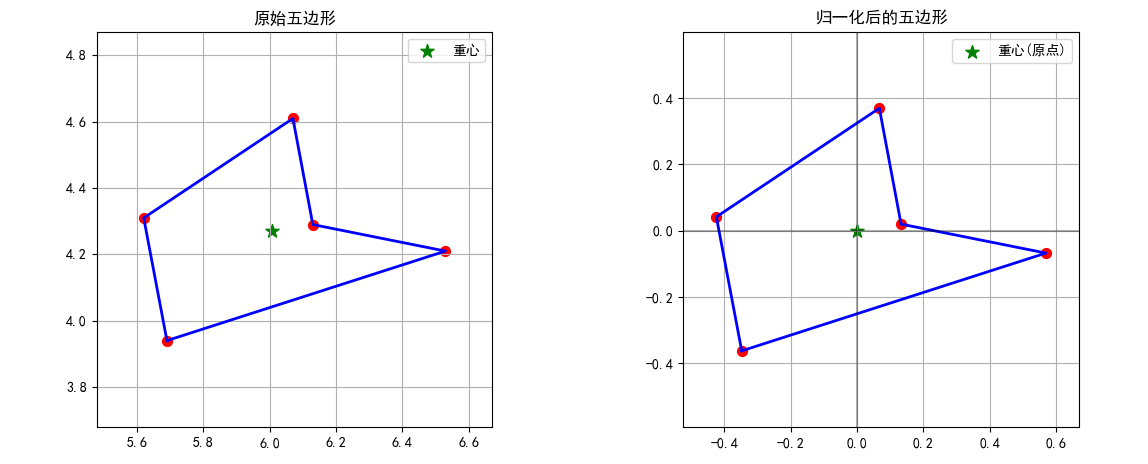
\includegraphics[width=1\textwidth]{figures/pentagon_normalization.png}

    % 说明:
    % 1. figures/pentagon_normalization.png 是您的图片文件相对于 .tex 文件的路径。
    % 2. [width=0.8\textwidth] 是一个可选参数,用于设置图片的宽度。
    %    0.8\textwidth 表示图片宽度为当前文本宽度的 80%。
    %    您可以根据需要调整这个值。
    \caption{xxx示例}
    \label{fig:normalize} % \label 必须放在 \caption 之后或内部,以便正确引用
\end{figure}

\subsubsection{xxxx模型的建立}

% 注意, 模型一般是数学公式, 少数情况可以是图形(常用图论求解时会用到)+一个算法(算法要写伪算法或给出流程图). 
% 但不能是纯文字说明. 下附算法的模板供参考. 在建模的过程,应该有必要的推理、推导、演算等. 
% 模型建立的叙述非常重要, 同学们往往是思路有了, 却怎么也交代不清楚,甚至觉得无话可说. 
% 大家要多看, 多写, 多思考才能写好. 我建模组老师也会尽量做到多给大家修改.
% 多看: 就是要多看优秀论文, 模仿优秀作品的写法先.
% 多练: 就是要多做题, 写完整的论文. 练一次, 写作能力就会提高一级.
% 多想: 就是要想想别人的文章好, 自己的不好, 差距在哪里?别人的文章还能不能改进, 写得更好. 
% 如果是几个模型, 采用格式:
% 1. ××××××模型
% ××××××××
% 2. ××××××模型
% ××××××××
% 3. ××××××模型
% ××××××××
在此处描述模型的建立过程,包括必要的推理、推导、演算等。
例如,可以定义模型的目标函数、约束条件等:
\begin{equation}
    \min f(x) = \sum_{i=1}^{n} c_i x_i \label{eq:obj_func_q1}
\end{equation}
约束条件:
\begin{align}
    \sum_{j=1}^{m} a_{ij} x_j \leq b_i, \quad & \forall i = 1, \dots, k \\
    x_j \geq 0, \quad & \forall j = 1, \dots, m
\end{align}
% 如果有算法,请使用伪代码或流程图描述。

\begin{algorithm}[H] % [H] 选项来自 float 宏包
\caption{五边形归类判别算法}
\label{alg:polygon_classification}
\begin{algorithmic}[1] % [1] 表示显示行号
    \Function{ClassifyPolygon}{$P, \mathit{ClassI}, \mathit{ClassII}$}
        \State 对输入的待测五边形$P$、类别I模板$\mathit{ClassI}$、类别II模板$\mathit{ClassII}$进行归一化处理
        \State 提取$P$的几何不变量特征向量$\mathcal{F}_P$
        \State 提取$\mathit{ClassI}$的几何不变量特征向量$\mathcal{F}_I$
        \State 提取$\mathit{ClassII}$的几何不变量特征向量$\mathcal{F}_{II}$
        \State 计算$P$与$\mathit{ClassI}$的特征向量欧氏距离 $d_{\mathcal{F},I} = \|\mathcal{F}_P - \mathcal{F}_I\|_2$
        \State 计算$P$与$\mathit{ClassII}$的特征向量欧氏距离 $d_{\mathcal{F},II} = \|\mathcal{F}_P - \mathcal{F}_{II}\|_2$
        \State 尝试所有可能的顶点对应和旋转,使用Kabsch算法计算$P$与$\mathit{ClassI}$和$\mathit{ClassII}$之间的最优刚性配准,得到$\mathit{RMSD}_{I}$和$\mathit{RMSD}_{II}$
        \State 计算$P$与$\mathit{ClassI}$的综合相似度评分 $S_I = \alpha \cdot \mathit{RMSD}_I + (1-\alpha) \cdot d_{\mathcal{F},I}$ 
        \State 计算$P$与$\mathit{ClassII}$的综合相似度评分 $S_{II} = \alpha \cdot \mathit{RMSD}_{II} + (1-\alpha) \cdot d_{\mathcal{F},II}$
        \If{$S_I < S_{II}$ \textbf{and} $S_I < \lambda$} \Comment{$\lambda$为预设阈值}
            \State \Return 类别I
        \ElsIf{$S_{II} < S_I$ \textbf{and} $S_{II} < \lambda$}
            \State \Return 类别II
        \Else
            \State \Return 未知类别
        \EndIf
    \EndFunction
\end{algorithmic}
\end{algorithm}


\subsubsection{模型的求解和分析}
    
    \textbf{1. 计算方法的选取or设计}
    
    为解问题一××××××模型,主要采用了××××××××算法。
    % 比较复杂的程序要写算法或者流程图(但是不要在正文中出现代码,代码一律在附件里)。
    
    \textbf{2. 参数的确定}
    
    对所建模型中参数是如何确定的,写出过程和具体的值。例如
    确定上述公式(\ref{eq:obj_func_q1})中的参数见表\ref{tab:params_q1}. 
    % 需要自行创建该表格
    
   \begin{table}[H]
    \centering
    \caption{五边形归类结果}
    \label{tab:params_q1}
    % --- 使用混合列类型 ---
    \begin{tabularx}{\textwidth}{ c c c c c C c } %<-- 核心修改

    \toprule
    \textbf{图形编号} & \textbf{RMSD\textsubscript{I}} & \textbf{RMSD\textsubscript{II}} & \textbf{$d_{\mathcal{F},I}$} & \textbf{$d_{\mathcal{F},II}$} & \textbf{综合评分(I/II)} & \textbf{归类结果} \\
    \midrule
    1 & 0.0082 & 0.2956 & 0.3220 & 6.5186 & 0.0578 / 1.2782 & 类别I \\
    2 & 0.3010 & 0.0160 & 6.7958 & 0.4994 & 1.3265 / 0.0924 & 类别II \\
    3 & 0.1812 & 0.2235 & 4.4074 & 5.5873 & 0.8485 / 1.0704 & 未知类别 \\
    4 & 0.0101 & 0.2937 & 0.3142 & 6.5064 & 0.0581 / 1.2747 & 类别I \\
    5 & 0.3010 & 0.0489 & 7.8076 & 1.6174 & 1.4862 / 0.2965 & 类别II \\
    \bottomrule
    \end{tabularx}
\end{table}

    \textbf{3. 计算结果}
    
    将确定的参数代入模型(公式\ref{eq:obj_func_q1}),运用×××软件的什么命令, 或自己编写的程序(程序见附录×), 得到怎样的结果. 
    % (结果展示以表格和图为好)

    \textbf{4. 结果分析}
    
    从图×或表×可以看出:×××××××××××××××(单调性,极值,最值,拐点). 结论是什么(定性结果:变好、变坏,增加、减少).
    
    \textbf{5. 问题一的回答}
    
    利用计算结果,逐一回答问题一提出的每一个问题。对随时间变换的量,建议给出时间变换曲线图。


\subsubsection{模型检验或修正}
说明假设合理性,说明在前文的假设下结果的正确性(合理性), 诸如此类.可以通过对误差进行分析(如,做仿真模拟), 提出修改假设和对模型的修正。
××××××
\subsection{问题二的建模与求解}
% 简短的概述, 问题二主要要解决什么问题, 建立了××××××模型, 用了什么方法解决. 
% 写出本小节主要内容(比如:本小节主要内容是数据的预处理、××××××模型的建立、模型的求解和分析、模型检验).
问题二主要解决 ×××××× 问题,为此建立了 ×××××× 模型, 采用了 ×××××× 方法进行求解。
本小节主要内容包括:数据的预处理、××××××模型的建立、模型的求解和分析、模型检验或修正。

\subsubsection{数据的预处理(如果是做数据多的题, 一定要写这一块; 不需要的就不做.)}
    \textbf{1. 数据的采集}
    
    ××××××××
    
    \textbf{2. 去噪处理}
    
    ××××××××
    
    \textbf{3. 数据的整理(如不全的数据要补全, 有的是要转化数据类型, 等等)}
    
    ××××××××

\subsubsection{××××××模型的建立 (在此处为模型命名)}
    % 这一目给大家介绍编辑文字的注意事项:
    % 1. 中文用宋体, 正体, 小四号, 见图2. 数字和英文用Times new Roman. 
    %    变量, 函数, 公式一律用公式编辑器(Mathtype)编写(公式编辑器的默认小四号中文对应英文变量为Times new Roman, 斜体, 12.5号). 
    %    实际上, 数字最好也用公式编辑器, 整体效果会比较好. 
    %    如果在公式中要强调某个变量是向量或矩阵, 则要用Times new Roman, 粗体+斜体, 12.5号. 
    %    (a.txt中的图2是Word字体设置截图,此处为LaTeX注释)
    % 2. 行距用单倍行距. 或控制在固定值16, 和单倍行距效果相似. 
    %    (a.txt中的图3是Word行距设置截图,此处为LaTeX注释)
    % 3. 段落间有间距比较好看. 建议段前0.5倍行距. 
    % 4. 公式编辑器的调用:插入→对象→MathType→确定
    %    (a.txt中的图4是Word公式编辑器调用截图,此处为LaTeX注释)
    %    也可以直接将word文档里现有的公式编辑器编写的公式, 如 $E=mc^2$, 复制, 粘贴到需要的位置, 再双击打开, 编写. 
    % 注意公式一般有两种:隐式和显式. 隐式一般比较短小, 写在文字中间即可.
    % 显式是比较大或者要重点强调的公式, 要单独一行居中. 
    % 后面需要用到的公式还要编号. 如:
    % 相邻节点 $v_i$ 和 $v_{i+1}$ 之间满足关系式:
    % \begin{equation}
    %     y_{i+1} = A y_i + B u_i \label{eq:state_space_q2}
    % \end{equation}
    % 其中, $A, B$ 是系数矩阵, $u_i$ 是控制输入.
    在此处描述问题二的模型建立过程。
    例如:
    \begin{equation}
        \frac{d\mathbf{x}}{dt} = f(\mathbf{x}(t), \mathbf{u}(t), t) \label{eq:q2_model}
    \end{equation}
    其中 $\mathbf{x}$ 是状态向量, $\mathbf{u}$ 是控制向量。

\subsubsection{模型的求解和分析}
    \textbf{1.参数的确定与模型求解}
    
    通过xx方法,确定公式(\ref{eq:q2_model})中的参数. 运用×××软件的什么命令, 或自己编写的程序(程序见附录×), 得到怎样的结果. 结果展示除数据公式外也可利用图或表. 
    
    \textbf{2. 结果分析}
    
    从图×或表×可以看出:×××××××××××××××. 结论是什么.
    从图×或表×可以看出:×××××××××××××××(单调性,极值,最值,拐点). 结论是什么(定性结果:变好、变坏,增加、减少).
    
    \textbf{3. 问题二的回答}
    
    利用计算结果,逐一回答问题二提出的每一个问题。对随时间变换的量,建议给出时间变换曲线图。

\subsubsection{模型检验或修正}
说明假设合理性,说明在前文的假设下结果的正确性(合理性), 诸如此类.可以通过对误差进行分析(如,做仿真模拟), 提出修改假设和对模型的修正。
××××××

\section{模型的检验/敏感性分析}
\subsection{模型的检验}
% 应进行模型检验。例如:对题目所给的数据加随机误差,考察模型的稳定性;考察重要参数对结果的影响等。
在此处描述模型的检验过程和结果。××××××

\subsection{敏感性分析}
% 可通过误差分析,找出敏感因子,&/or作全局敏感性分析(比如采用Sobol法)
在此处描述模型的敏感性分析过程和结果。××××××
\section{模型的评价与推广}
\subsection{模型的优点}
针对问题1 ××××××××××××

针对问题2 ××××××××××××

针对问题3 ××××××××××××

\subsection{模型的缺点}
针对问题1 ××××××××××××

针对问题2 ××××××××××××

针对问题3 ××××××××××××

\subsection{模型的推广}
××××××××××××

%%%%%%%%%%%%%%%%%%%%%%%%%%%%%%%%%%%%%%%%%%%%%%%%%%%%%%%%%%%%%
%% 参考文献

\nocite{*} % 引用所有.bib文件中的条目,即使未在正文中\cite
\bibliographystyle{gbt7714-numerical}  % 引用格式,符合GB/T 7714-2015数值引用
\bibliography{ref}  % bib源文件名 (ref.bib)
% 请确保您有一个名为 ref.bib 的文件,并在其中按上述格式或标准BibTeX格式管理您的参考文献。

\newpage
%%%%%%%%%%%%%%%%%%%%%%%%%%%%%%%%%%%%%%%%%%%%%%%%%%%%%%%%%%%%%
\phantomsection    % 为 hyperref 创建正确的锚点,使得目录中的“附录”可点击
\addcontentsline{toc}{section}{附录} % 将“附录”作为 section 级别添加到目录
                                                  % 你可以调整字体大小和粗细
\begin{appendices} % 开始附录环境
    % 这个环境会在目录中添加"附录"这一行,并在正文打印"附录"大标题。
    

\begin{table}[H]
\centering
% 列定义:最左、最右有竖线,并且在第一列和第二列之间,第二列和第三列之间也有竖线
\begin{tabularx}{\linewidth}{| >{\centering}p{0.15\linewidth} | L | L |} % <--- 修改列定义
\toprule
% 跨三列的“附录清单”标题,左右也应该有竖线以匹配表格外框
\multicolumn{3}{|c|}{\textbf{\Large 附录清单}} \\ % 注意这里multicolumn的格式调整为 c| 或 |c| 或 |c
                                                % 更精确的应该是 |c| 如果左右都有线
                                                % 但由于它已经是最外层,tabularx的 | 会处理外框
                                                % 不过,为了清晰,且如果下面有内部竖线,
                                                % 通常 \multicolumn 也需要指定其内部竖线。
                                                % 这里因为附录清单下面没有内部竖线,所以 c 就可以。
                                                % 但为了应对下一行的竖线,我们让它也匹配竖线模式
\midrule
% 列标题,列与列之间有竖线
\textbf{附录编号} & \textbf{名称} & \textbf{解释} \\ % 这里的 & 会自动在它们之间画线 (基于上面的 |L|L|)
\midrule
附录A & 可视化函数(部分) & 可视化数据 \\
\midrule % 在每个数据行后加一条水平线,以模仿你图片中每行都有分隔的效果
附录B & 问题一:五边形分类代码(主要逻辑) & q1.py 文件中与五边形分类相关的核心类和函数定义 \\
\midrule
附录C & 问题二:八面体分类代码(主要逻辑) & q2.py 文件中与八面体分类相关的核心类和函数定义 \\
\bottomrule
\end{tabularx}
\end{table}
    
\subsection*{附录A: 可视化函数}
    
\noindent visual.py
\lstinputlisting[language=python,basicstyle=\ttfamily\small]{code/visual.py}
    
\subsection*{附录B: 问题一五边形分类核心代码}
    
\noindent q1.py
\lstinputlisting[language=python, basicstyle=\ttfamily\small]{code/q1.py}

\subsection*{附录C: 问题二八面体分类核心代码}
    
\noindent q2.py
\lstinputlisting[language=python,  basicstyle=\ttfamily\small]{code/q2.py}
    
\end{appendices} % 结束附录环境
\newpage


\end{document}